\setcounter{section}{0}

\section{P vs. NP}
One provides a solution to 
the Boolean satisfiability 
problem.
\begin{center}
  \begin{verbatim}
  True=1, False=1
  \end{verbatim}
\end{center}
One verifies 
the satisfiability 
of any formula in $O(1)$ time.
\begin{center}
  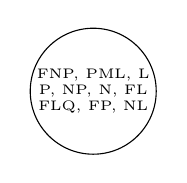
\begin{tikzpicture}[scale=0.2pt]
    \draw (0,0) circle (4);
    \node at (0,0) {\tiny P, NP, N, FL};
    \node[below] at (0,0) {\tiny FLQ, FP, NL};
    \node[above] at (0,0) {\tiny FNP, PML, L};
  \end{tikzpicture}
\end{center}

% picture of NP, P, L, etc.. complexities, but they all overlap

